\documentclass[pre,preprint,superscriptaddress]{revtex4-1} 

\usepackage{graphicx}
\usepackage{hyperref}
\usepackage{amsmath}
\usepackage{amsfonts} % needed for bold Greek, Fraktur, and blackboard bold
\usepackage{amssymb}
\usepackage[margin=1in]{geometry}
\usepackage{dcolumn}
\usepackage{multirow}
\usepackage{tikz}
\usetikzlibrary{calc,patterns,decorations.pathmorphing,decorations.markings}
\usepackage{hyperref}
\usepackage{float}
\usepackage{subfig}
\usepackage{todonotes}
\usepackage{subfiles}

% TODO: remove these lines, which expand the margins (useful for comments)
\textwidth  .72\paperwidth
\hoffset -1in
\oddsidemargin .14\paperwidth
\evensidemargin .14\paperwidth
\marginparwidth .11\paperwidth


% Draft macros
\usepackage[normalem]{ulem} % for strikethrough
%\usepackage[usenames,dvipsnames]{xcolor}
%\newcommand{\TODO}[1]{\marginpar{\raggedright\scriptsize\textbf{TODO:} #1} (\textbf{TODO})}
%\newcommand{\NOTEMARG}[1]{\marginpar{\raggedright\scriptsize\textbf{NOTE:} #1} (\textbf{NOTE})}
%\newcommand{\NOTE}[1]{\marginpar{\footnotesize\textbf{NOTE}} (\textbf{NOTE: #1})}
%\definecolor{purple}{rgb}{1,0,1}


\newcommand{\eq}[1]{eq.~\eqref{eq:#1}}
\newcommand{\eqs}[2]{eqs.~\eqref{eq:#1} and \eqref{eq:#2}}
\renewcommand{\sec}[1]{section~\ref{sec:#1}}
\newcommand{\secs}[2]{sections~\ref{sec:#1} and \ref{sec:#2}}
\newcommand{\subsec}[1]{section~\ref{subsec:#1}}
\newcommand{\subsubsec}[1]{section~\ref{subsubsec:#1}}
\newcommand{\app}[1]{appendix~\ref{app:#1}}
\newcommand{\fig}[1]{figure~\ref{fig:#1}}
\newcommand{\figs}[2]{figures~\ref{fig:#1} and \ref{fig:#2}}
\newcommand{\tab}[1]{table~\ref{tab:#1}}
\newcommand{\nn}{\nonumber}




\begin{document}

\title{Time dependent forcing in the Swift-- Hohenberg equation}
\author{Punit Gandhi}
 \email{punit\_gandhi@berkeley.edu}
\author{C\'edric Beaume}
\author{Edgar Knobloch}
 \email{knobloch@berkeley.edu}
\affiliation{Department of Physics, University of California, Berkeley CA 94720, USA}
\date{\today}

\begin{abstract}
This is an update of some results we've found and don't understand yet regarding the structure of the stable region in parameter space of oscillation frequency and center of oscillation while fixing the amplitude of oscillation.  We also discuss some issues we've encountered while calculated the speed of the front.
\end{abstract}

\maketitle

\section{Introduction}
The equation we consider is: 
\begin{equation}
u_t= (r_0+ \rho \sin\omega t) u-\left(1+\partial_{x}^2\right)^2u+u^2-u^3\label{eq:SH},
\end{equation}
which describes the dynamics of a real field $u$ over one spatial dimension in time.  We have rescaled the equation so that the critical wavenumber that defines the natural wavelength of the patterned state is unity.   The average value of the linear forcing term $r_0$, the amplitude of oscillation $\rho$, the frequency of oscillation $\omega$, and the strength quadratic/cubic nonlinearity $b$ are left as parameters of the system.  We will, however, fix $b=1.8$ and focus mostly on $\rho =0.1$ thoughout this note.    

\section{bistability and localized solutions in SHE}
The caption of Fig.~\ref{fig:BurkeSHE}  taken from J. Burke et et al., describes the locations of bifurcations and relevant boundaries of the constant forcing version of this problem ( e.g. $\rho=0$) with $b=1.8$.  

\begin{figure}[h!]\center
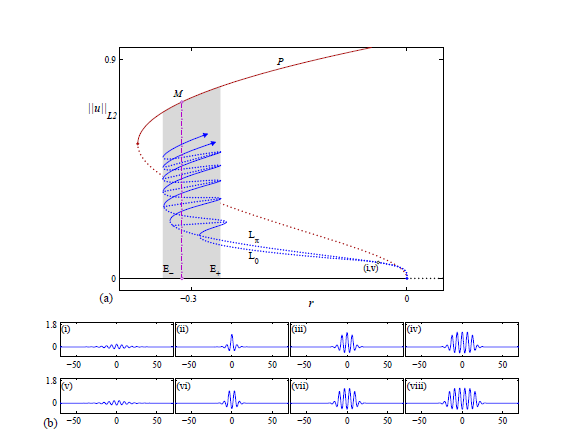
\includegraphics[width=120mm]{BurkeSHE.PNG}
\caption{\label{fig:BurkeSHE}This figure was taken from Burke\cite{} (a) Bifurcation diagram showing the snakes-and-ladders structure of localized states. Away from the origin the snaking branches $L_0$ and $L_-$ are contained within the snaking region (shaded) between$E_-$ and $E_+$, where $r(E_-)\approx -0.3390$ and $r(E_+)\approx -0.2593$.   Solid (dotted) lines indicate stable (unstable) states. In addition, the Maxwell point $M$, occurring at $r(M)\approx -0.3128$  is indicated with a vertical dash-dot line.  The saddle node bifurcation that creates the stable periodic state occurs at $r<r(SN_P)\approx -0.3744$, defining the left edge of the bistability region.  We will also find it useful to define the center of the snaking region $C$, which corresponds to  the forcing parameter $r(C)\approx -0.2992$. (b) Sample localized profiles $u(x): (i-iv)$ lie on $L_0$, near onset and at the 1st, 3rd, and 5th saddle-nodes from the bottom, respectively; (v-viii) lie on $L_-$, near onset and at the 1st, 3rd, and 5th saddle-nodes, respectively. Parameters: $b = 1.8$.} 
\end{figure}


\section{Numerical results}

All simulations in time used periodic boundary conditions and a domain of $L=80\pi$ (e.g. 40 characteristic wavelengths).  A 4th order exponential time differencing scheme\cite{cox2002} was used to step forward  in time while spectral methods on a grid of 1024 points were used for the spatial calculations.  Steady state solutions were computed by numerical continuation using AUTO~\cite{doedel1981auto}.   We will focus on SHE23 case with $b=1.8$ and will always initialize the problem with a stable localized solution that fills roughly half the domain, and has been time-stepped with a constant forcing of $r_0$ to ensure it is a stable at this forcing value.  We can vary the way the forcing oscillates ($r\rightarrow r_0+\rho \sin\omega t$) in 3 ways: (1) the amplitude of the oscillation, $\rho$ (2) the point about which the oscillation occurs, $r_0$ (3) the frequency with which the oscillation occurs, $\omega$. 

\subsection{Front speed of constant forcing problem}
Burke and Knobloch \cite{burke2006}  have shown that near the snaking region (e.g. for $r=r(E_{\pm})\pm\delta$ where $\delta <<1$), a localized solution will move towards the more energetically favorable of the trivial and the periodic state.  Above the snaking region, for example, a localized solution will nucleate periods of the pattern in quick bursts with some longer transition time $T_{nuc}\propto \delta^{-1/2}$ in between each nucleation event.  We show the results of simulations to numerically confirm the region of validity of this law for our parameters in Fig.~\ref{fig:nucleation}.  We also show a graph of the front speed (calculated as $2 \pi / T_{nuc}$) as a function of $r_0$ for the constant forcing case.   It is clear from these graphs, that the front moves faster to the left of pinning region in the parameter regime we are looking at.  We also note that beyond $\delta$ of about 0.036, our algorithm fails to distinguish nucleation events to the left of the pinning region because they are no longer clearly separated by a period of slow change in the solution.  With an amplitude of oscillation of $\rho = 0.1$, the system actually reaches above this cutoff for most of the $r_0$ values we scan over.   


 \begin{figure}[h!]
  \begin{center}
    \mbox{
      \subfloat[]{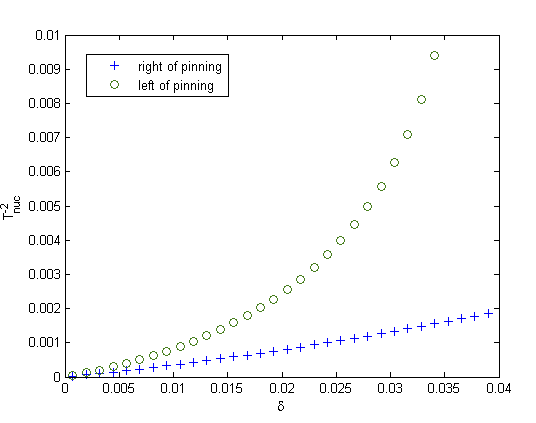
\includegraphics[width=60mm]{NucleationTime.png}} \quad
      \subfloat[]{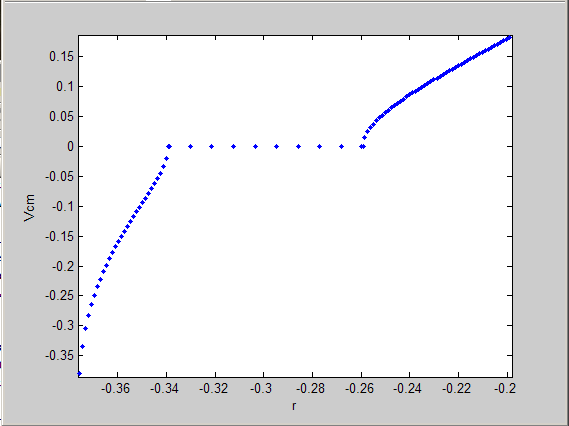
\includegraphics[width=60mm]{FrontSpeed.png} }
      }
    \caption{Simulation of the SHE with $N_{23}$ with $b=1.8$ show (a) $1/T_{nuc}^2$, where $T_{nuc}$ is the time between nucleation/decay events as a function of distance from the edge of the pinning region, and (b) the front speed as a function of the forcing parameter. We note that the initial solution used in these simulations was on a saddle node bifurcation of snaking branch at the closest edge of the pinning region.}
    \label{fig:nucleation}
  \end{center}
\end{figure} 



\subsection{oscillations around the pinning region}
We explore what happens in the case that you start with a steady state solution within the pinning region, but oscillate the forcing parameter about the pinning region. Figure~\ref{fig:Vcm01} show some results from a scan of the parameter space over the period of oscillation $T_{osc}$, and the average value of forcing $r_0$ with a fixed amplitude of oscillation, $\rho =0.1$.  We track the front of solution in terms of its first moment:
\begin{equation}
X_{cm}=\frac{1}{||u||} \int_{L/2}^{L/2}  |x| |u|^2 dx
\end{equation}
where 
\begin{equation}
||u||= \int_{L/2}^{L/2}  |u|^2 dx
\end{equation}
This give half the distance from the center of the domain to the edge of a localized solution. The speed is then defined by $V_{cm} = d X_{cm}/dt$, and is really half the speed of the front.


\begin{figure}[h!]\center
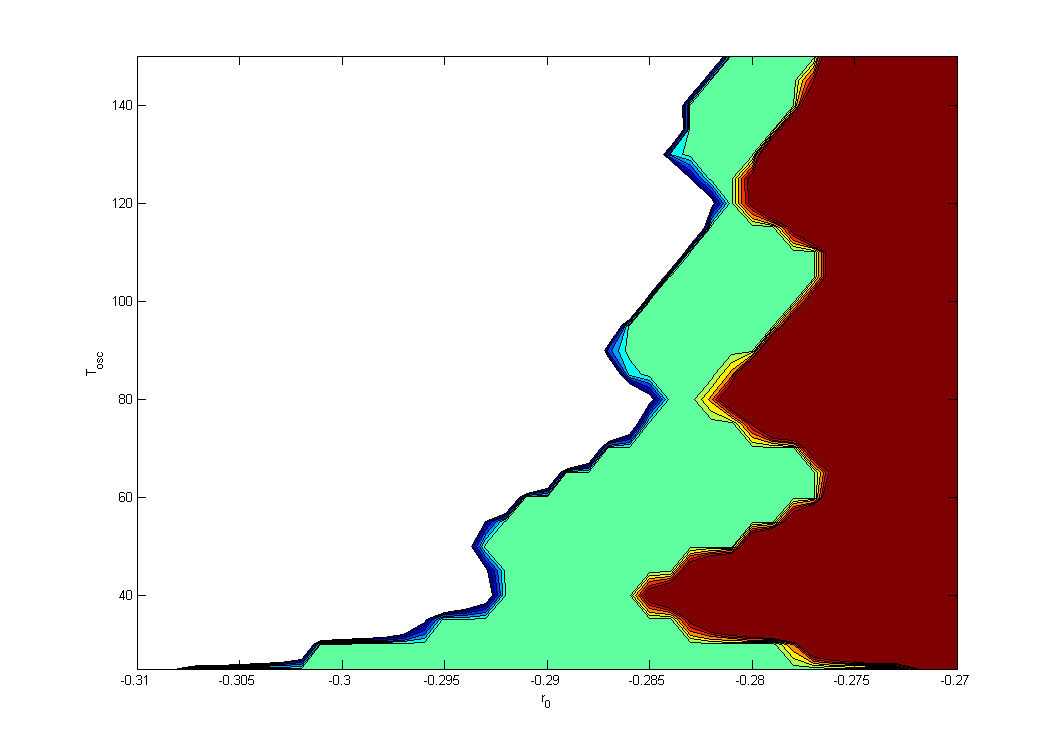
\includegraphics[width=120mm]{Vcm01.png}
\caption{The average speed at which the solution grows or decays as a function of oscillation period and oscillation center of the forcing parameter when $\rho=0.1$.  The solution had decayed by 6 or more periods over the course of the simulation (2000 units of time) in the white region, and has grown by six or more periods over the course of the simulation  in the red region.  The green region indicates where the solution has not grown or decayed on average.}
    \label{fig:Vcm01}
\end{figure}

We note that changing the phase of the oscillation in the forcing (e.g. $\rho\rightarrow-\rho$) does not seem to affect the stable region in this graph, but we need to do more work to confirm this is the case.  In order to explore the small scale bumpiness, we have zoomed in to a smaller region of parameter space with a finer mesh.  The results are shown in Fig.~\ref{fig:Vcm01zoom}.  We suspect that this bumpiness is due to the representation and grid approximation, and are working to smooth it out.
\begin{figure}[h!]\center
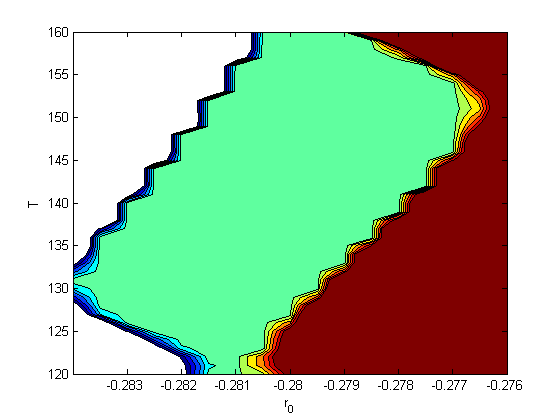
\includegraphics[width=120mm]{Vcm01zoom.png}
\caption{The average speed at which the solution grows or decays as a function of oscillation period and oscillation center of the forcing parameter.  The solution had decayed by 6 or more periods over the course of the simulation (2000 units of time) in the white region, and has grown by six or more periods over the course of the simulation  in the red region.  The green region indicates where the solution has not grown or decayed on average.}
    \label{fig:Vcm01zoom}
\end{figure}


To give a better sense of what is happening, we show the solution as a function of time for a series of simulations at a fixed $r_0=-.28$ and different oscillation times. Figures~\ref{fig:r28slice1} and \ref{fig:r28slice2} show both the solution and $Xcm$ for oscillation periods $T_{osc}=20,40,60,80$.  For these parameters, the solution oscillates between growing and stable. For larger oscillation periods ($T_{osc} \approx 200$), the solution transitions to going between stable and decaying as shown in Fig.~\ref{fig:r28slice3}.  
 \begin{figure}[h!]
  \begin{center}
    \mbox{
      	\subfloat[]{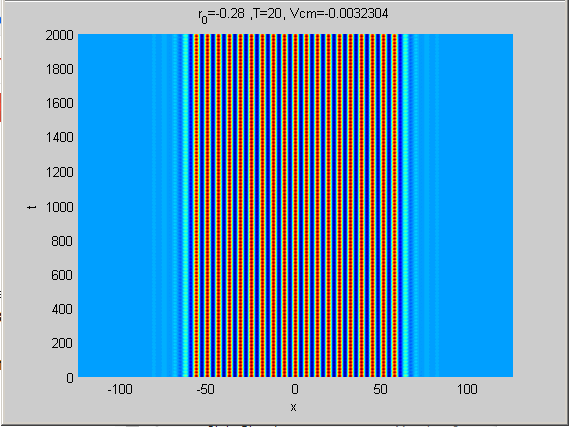
\includegraphics[width=60mm]{r0nD28drD10t020sol.png}}\quad 
      	\subfloat[]{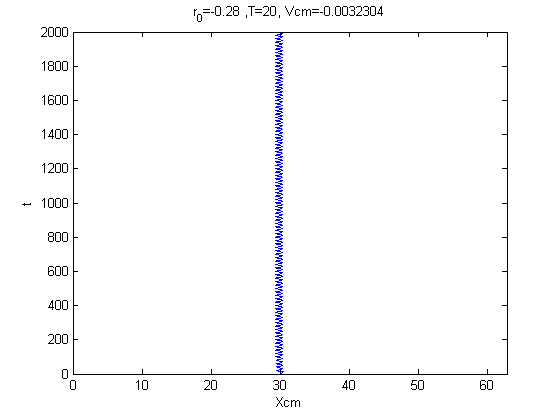
\includegraphics[width=60mm]{r0nD28drD10t020Xcm.png}} 
      } \mbox{
      	\subfloat[]{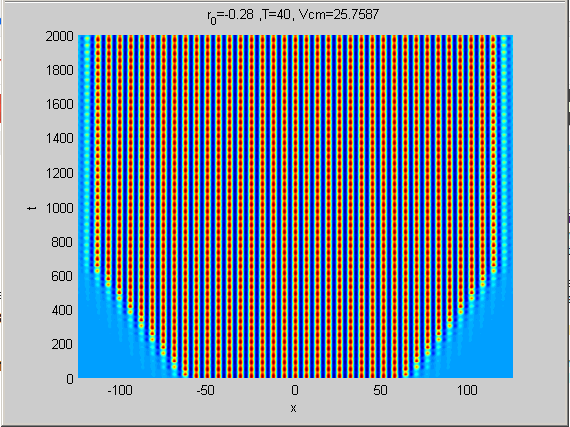
\includegraphics[width=60mm]{r0nD28drD10t040sol.png} }\quad 
	\subfloat[]{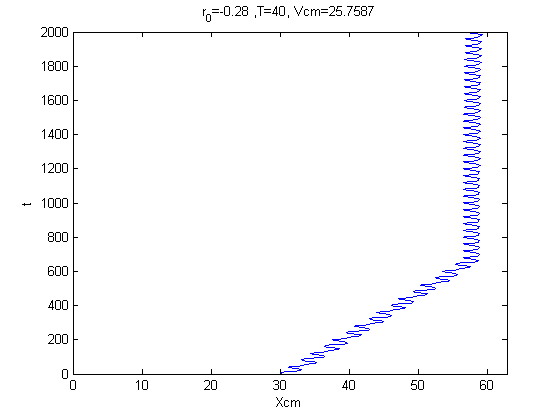
\includegraphics[width=60mm]{r0nD28drD10t040Xcm.png} }
      }
    \caption{Solutions along with Xcm are shown as  function of time for a series of oscillation periods at a fixed value of $r_0=-0.28$.  We see that the solution oscillates between growing and stable for this region, as expected given Fig.~\ref{fig:Vcm01}.  The value of $V_{cm}$ is given in number of periods nucleated or decayed over the course of the simulation (2000 units of time), assuming no boundary.}
    \label{fig:r28slice1}
  \end{center}
\end{figure} 

 \begin{figure}[h!]
  \begin{center}
        \mbox{
	\subfloat[]{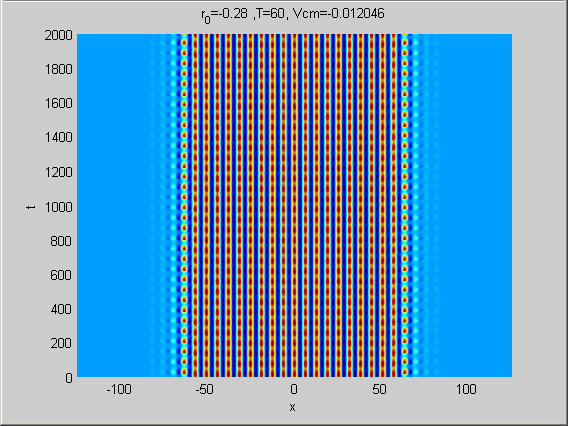
\includegraphics[width=60mm]{r0nD28drD10t060sol.png} }\quad 
	\subfloat[]{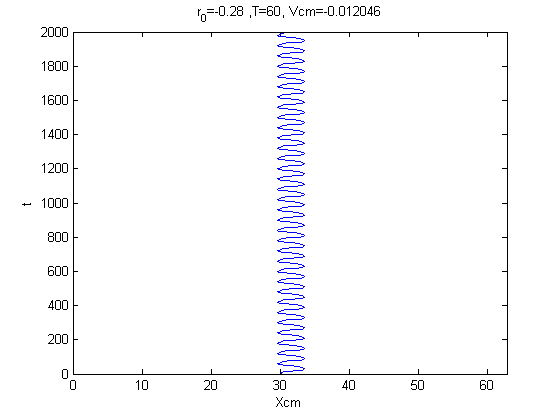
\includegraphics[width=60mm]{r0nD28drD10t060Xcm.png} }
      } \mbox{
	\subfloat[]{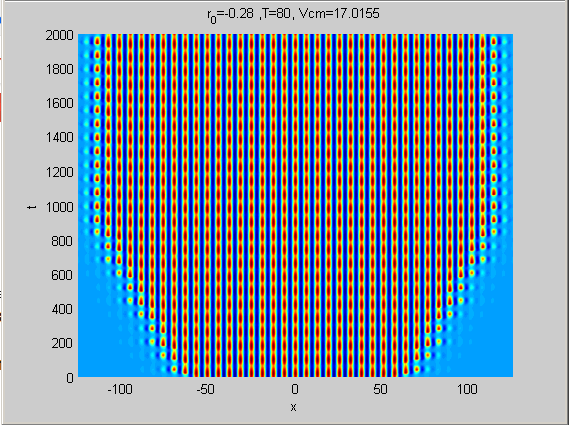
\includegraphics[width=60mm]{r0nD28drD10t080sol.png} }\quad
	\subfloat[]{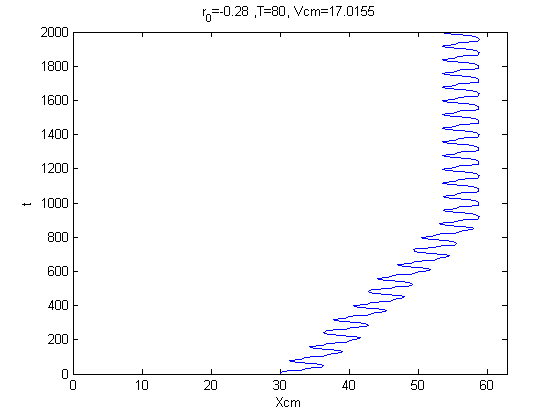
\includegraphics[width=60mm]{r0nD28drD10t080Xcm.png} }
      }
    \caption{Solutions along with Xcm are shown as  function of time for a series of oscillation periods at a fixed value of $r_0=-0.28$.  We see that the solution oscillates between growing and stable for this region, as expected given Fig.~\ref{fig:Vcm01}.  The value of $V_{cm}$ is given in number of periods nucleated or decayed over the course of the simulation (2000 units of time), assuming no boundary.}
    \label{fig:r28slice2}
  \end{center}
\end{figure} 
For the growing solutions, we see that the pattern of growth can occur over a different number of oscillations of the forcing and this may be related to the large scale oscillations in the boundary of the stable region shown in Fig.~\ref{fig:Vcm01}.  We see, for example, a nucleation event every oscillation period at $T_{osc}=40$ , but two nucleation events every three oscillations in the next growing solution at $T_{osc}=80$.
  \begin{figure}[h!]
  \begin{center}
    \mbox{	
	\subfloat[]{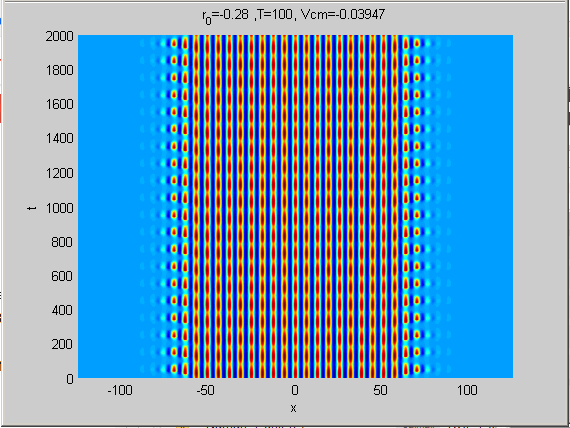
\includegraphics[width=60mm]{r0nD28drD10t100sol.png} }\quad 
	\subfloat[]{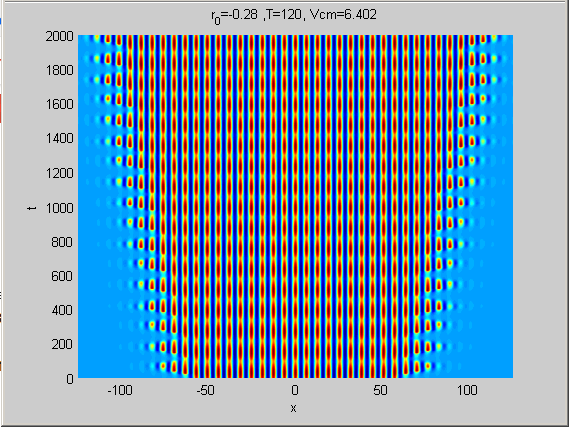
\includegraphics[width=60mm]{r0nD28drD10t120sol.png} } 
      } \mbox{
	\subfloat[]{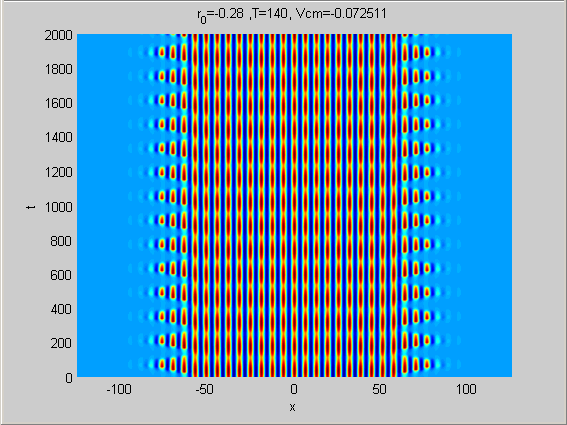
\includegraphics[width=60mm]{r0nD28drD10t140sol.png} }\quad 
	\subfloat[]{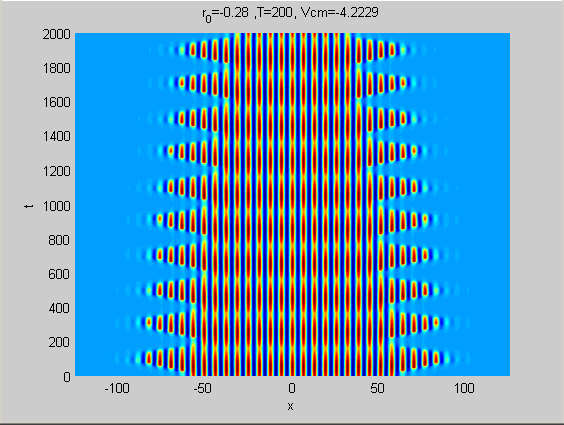
\includegraphics[width=60mm]{r0nD28drD10t200sol.png} } 
      }
    \caption{The pattern of oscillating between stable and growing solution continues up to about $T_{osc}=140$ and then, after a longer region of stability, the solutions oscillate between stable and decaying. The value of $V_{cm}$ is given in number of periods nucleated or decayed over the course of the simulation (2000 units of time), assuming no boundary.}
    \label{fig:r28slice3}
  \end{center}
\end{figure} 



We have also done very preliminary calculations on $\rho =0.06$ (shown in Fig.~\ref{fig:Vcm006}), and have found that it seems to stretch graph out vertically so that you need a longer period to see the same qualitative features.  This makes sense given that a smaller oscillation amplitude means less time outside of the snaking region.   


\begin{figure}[h!]\center
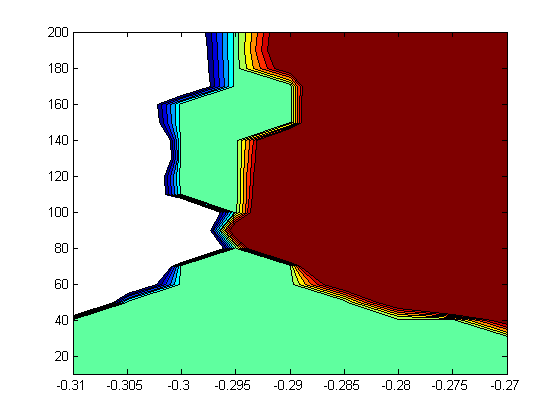
\includegraphics[width=120mm]{Vcm006error.png}
\caption{The average speed at which the solution grows or decays as a function of oscillation period and oscillation center of the forcing parameter when $\rho=0.06$.  The solution had decayed by 6 or more periods over the course of the simulation (2000 units of time) in the white region, and has grown by six or more periods over the course of the simulation  in the red region.  The green region indicates where the solution has not grown or decayed on average.}
    \label{fig:Vcm006}
\end{figure}


We note that our data on the front speed shown in Fig.~\ref{fig:nucleation} stretches far enough to cover all of the forcing parameters that are sampled during the simulations here. Given the speed of the front as a function of the forcing parameter, $V_0(r)$ ,  We numerically determine a ``break-even" point were we would not expect the front to move on average for a particular value of $r_0$.  We define $r_*$  by the condition that 
\begin{equation}
\int_0^{2\pi} V_{0} ( r_*+\rho \sin\phi) d\phi = 0.
\end{equation}
For $\rho =0.06$, we find that $r_*\approx -0.295$, which roughly corresponds to the center point of the stable region of Fig.~\ref{fig:Vcm006}.

\bibliography{TimeForcingSHE_bibliography}

\end{document}


